%~~~~~~~~~~~~~~~~~~~~~~~~~~~~~~~~~~~~~~~~~~~~~~~~~~~~~~~~~~~~~~~~~~~~~~~~~~~~~~~~~~~~~~~~~%
%~~~~~~~~~~~~~~~~~~~~~~~~~~~~~~~~~~~~~~~~~~~~~~~~~~~~~~~~~~~~~~~~~~~~~~~~~~~~~~~~~~~~~~~~~%
%	                  PREAMBLE (PACKAGES AND DOCUMENT CONFIGURATION)                      %
%~~~~~~~~~~~~~~~~~~~~~~~~~~~~~~~~~~~~~~~~~~~~~~~~~~~~~~~~~~~~~~~~~~~~~~~~~~~~~~~~~~~~~~~~~%

% Set the font size (in pt) and paper size (letterpaper, a4paper, etc)
\documentclass[12pt,a4paper]{report}

\oddsidemargin 0.5cm \evensidemargin 0.5cm
\marginparwidth 40pt \marginparsep 10pt
\topmargin 0pt \headsep 40pt
\textheight 635pt \textwidth 450pt

\usepackage{amsthm,amssymb,mathrsfs,setspace,booktabs}
\usepackage{mathtools,amsmath,nccmath}
\usepackage{pdfpages}



\usepackage[a4paper,top=0.75in,bottom=0.75in,left=0.75in,right=0.75in]{geometry}
\renewcommand{\baselinestretch}{1.15}
\usepackage{times}
\usepackage{titlesec}
\setlength{\parskip}{0.5em plus 0.1em minus 0.1em}
\setlength{\textheight}{\dimexpr\paperheight-2in}
\titlespacing*{\chapter}{0pt}{-20pt}{10pt}
\titlespacing*{\section}{0pt}{*1.0}{*0.5}
\titlespacing*{\subsection}{0pt}{*0.5}{*0.25}




% UNCOMMENT REQUIRED PACKAGES. 
% CAREFULLY REMOVE UNNECESSARY PACKAGES TO DECREASE COMPILE TIME.
% READ ALL ASSOCIATED PACKAGE HELP FILES BEFORE USE.

\usepackage{pstricks} % PSTricks offers an extensive collection of quick and easy macros for generating PostScript including macros for colour, graphics, pie charts, rotation, trees and overlays. (https://ctan.org/pkg/pstricks-base?lang=en)

\usepackage{tikz} % Used in Images/Figures/3D_Cone.tex, disable if not needed
% tikz package for drawing graphs and diagrams [XY-pic is now outdated]
% (https://ctan.org/pkg/tikz?lang=en)

%\usepackage{tikz-cd} % Commutative Diagrams with Tikz, primarily for linear algebra.
% (https://ctan.org/pkg/tikz-cd?lang=en)

%\usepackage{pgfplots} % pgfplots with tikz package is used to portray detailed 2D and 3D function plots and graph data with a high degree of customization. (https://www.overleaf.com/learn/latex/Pgfplots_package)
% (https://ctan.org/pkg/pgfplots?lang=en)

%\usepackage{footmisc} % footmisc package for more control over typesetting footnotes.
% (https://ctan.org/pkg/footmisc?lang=en)

\usepackage[%
    colorlinks=true,
    pdfborder={0 0 0},
    linkcolor=red    
]{hyperref} % hyperref package for creating reliable hyperlinks and referral links.
% (https://ctan.org/pkg/hypperref?lang=en)

\usepackage{appendix} % appendix package for appendix-related formatting.
% (https://ctan.org/pkg/appendix?lang=en)

%\usepackage{listofsymbols} % listofsymbols package for establishing a legend for any symbols used.
% (https://ctan.org/pkg/listofsymbols?lang=en)

\usepackage{caption} % caption package for better control over figure and table captions.
% (https://ctan.org/pkg/caption?lang=en)

%\usepackage{booktabs} % The booktabs package allows better control over tables including ruling, width, etc. (https://ctan.org/pkg/booktabs?lang=en) 

\usepackage[style=numeric,sorting=nyt]{biblatex}


\usepackage{fancyhdr} % fancyhdr package gives better control over headers and footers.
% (https://www.overleaf.com/learn/latex/Headers_and_footers)
%\pagestyle{fancy} % Enable for quick header and footer throughout your document.

\usepackage{multicol} % multicol package allows the use of columns in your documents.
% (https://ctan.org/pkg/multicol?lang=en)

\usepackage{geometry} % geometry package for absolute control over the dimensions of the usable space on a page.
% (https://ctan.org/pkg/geometry?lang=en)

\usepackage{xcolor} % xcolor package for better control over colours.
% (https://ctan.org/pkg/xcolor?lang=en)
\hypersetup{
    colorlinks,
    linkcolor={blue!50!black},
    citecolor={blue!50!black},
    urlcolor={blue!80!black}
}

\usepackage{graphicx} % Provides additional control over the \includegraphics command
% (https://ctan.org/pkg/graphicx)

\usepackage[nottoc]{tocbibind} % Adds LoF and LoT to ToC
%~~~~~~~~~~~~~~~~~~~~~~~~~~~~~~~~~~~~~~~~~~~~~~~~~~~~~~~~~~~~~~~~~~~~~~~~~~~~~~~~~~~~~~~~~%

\renewcommand{\chaptermark}[1]{\markboth{#1}{}}
\renewcommand{\sectionmark}[1]{\markright{\thesection\ #1}}

\setlength{\parskip}{1em plus 0.25em minus 0.25em}

\theoremstyle{plain}
\newtheorem{theorem}{Theorem}[section]
\newtheorem{lemma}[theorem]{Lemma}
\newtheorem{corollary}[theorem]{Corollary}
\newtheorem{proposition}[theorem]{Proposition}

\theoremstyle{definition}
\newtheorem{definition}[theorem]{Definition}
\newtheorem{example}[theorem]{Example}
\newtheorem{notation}[theorem]{Notation}

\theoremstyle{remark}
\newtheorem{remark}[theorem]{Remark}

\renewcommand{\baselinestretch}{1.5}



%~~~~~~~~~~~~~~~~~~~~~~~~~~~~~~~~~~~~~~~~~~~~~~~~~~~~~~~~~~~~~~~~~~~~~~~~~~~~~~~~~~~~~~~~~%
%                          Abbreviations, Constants and Symbols                           %
%~~~~~~~~~~~~~~~~~~~~~~~~~~~~~~~~~~~~~~~~~~~~~~~~~~~~~~~~~~~~~~~~~~~~~~~~~~~~~~~~~~~~~~~~~%

% Uncomment lines for enabling the use of abbreviations in 07_Abbrev,Const,Symbols.tex
\usepackage{longtable}
\newcommand\listsymbolname{Abbreviations}
\newcommand\tab[1][1cm]{\hspace*{#1}}
\newcommand\listofsymbols[2]{
\btypeout{\listsymbolname}
\addtotoc{\listsymbolname}
    \chapter*{\listsymbolname
      \@mkboth{
          \MakeUppercase\listsymbolname}{\MakeUppercase\listsymbolname}}
\begin{longtable}[c]{#1}#2\end{longtable}\par
    \cleardoublepage
}

% Uncomment lines for enabling the use of constants in 07_Abbrev,Const,Symbols.tex
%\newcommand\listconstants{Physical Constants}
%\newcommand\listofconstants[2]{
%\btypeout{\listconstants}
%\addtotoc{\listconstants}
%    \chapter*{\listconstants
%      \@mkboth{
%          \MakeUppercase\listconstants}{\MakeUppercase\listconstants}}
%\begin{longtable}[c]{#1}#2\end{longtable}\par
%    \cleardoublepage
%}

% Uncomment lines for enabling the use of symbols in 07_Abbrev,Const,Symbols.tex
%\newcommand\listnomenclature{Symbols}
%\newcommand\listofnomenclature[2]{
%\btypeout{\listnomenclature}
%\addtotoc{\listnomenclature}
%    \chapter*{\listnomenclature
%      \@mkboth{
%          \MakeUppercase\listnomenclature}{\MakeUppercase\listnomenclature}}
%\begin{longtable}[c]{#1}#2\end{longtable}\par
%    \cleardoublepage
%}

% Uncomment for some standard notations in math as required
% \displaystyle or \ds lets you switch back the display style to default, during,
% say, a cascading fraction 

%\DeclarePairedDelimiter\ceil{\lceil}{\rceil}
%\DeclarePairedDelimiter\floor{\lfloor}{\rfloor}
%\DeclarePairedDelimiter\norm{\left\lVert}{\right\rVert}
%\newcommand{\reals}{\mathbb R}
%\newcommand{\complex}{\mathbb C}
%\newcommand{\rational}{\mathbb Q}
%\newcommand{\int}{\mathbb Z}
%\newcommand{\nat}{\mathbb N}
%\newcommand{\jacobian}{\mathcal J}
%\newcommand{\bigzero}{\mbox{\normalfont\Large\bfseries 0}}
%\newcommand{\ds}{\displaystyle}
%\newcommand{\Ll}{\mathbb L}
%\newcommand{\la}{\lambda}
%\newcommand{\cof}{\textup{cof }}
%\newcommand{\dsum}{\displaystyle\sum}
%\newcommand{\1}{\mathbf 1}

\usepackage{minted}
\usepackage{titlesec}
\titleformat{\chapter}[hang]
{\normalfont\LARGE\bfseries}{\thechapter.}{1em}{\LARGE}
\titlespacing*{\chapter}{0pt}{-20pt}{20pt}

\addbibresource{ref.bib}

\begin{document}

%~~~~~~~~~~~~~~~~~~~~~~~~~~~~~~~~~~~~~~~~~~~~~~~~~~~~~~~~~~~~~~~~~~~~~~~~~~~~~~~~~~~~~~~~~%
% CUSTOM INPUT FIELDS ARE MARKED WITH [] IN THE INTRO SECTIONS.
% REWRITE INPUTS ACCORDING TO CAPITALIZATION WITHIN BRACKETS (First Letter Capital/ALL UPPERCASE/all small letters).
% GO THROUGH EACH INTRO PAGE AND UPDATE ALL OF YOUR PERSONAL INFORMATION ACCORDINGLY.
% READ ALL UNCOMMENTED LINES CAREFULLY.
%~~~~~~~~~~~~~~~~~~~~~~~~~~~~~~~~~~~~~~~~~~~~~~~~~~~~~~~~~~~~~~~~~~~~~~~~~~~~~~~~~~~~~~~~~%

%~~~~~~~~~~~~~~~~~~~~~~~~~~~~~~~~~~~~~~~~~~~~~~~~~~~~~~~~~~~~~~~~~~~~~~~~~~~~~~~~~~~~~~~~~%
%	                                     TITLE PAGE	                                      %
%~~~~~~~~~~~~~~~~~~~~~~~~~~~~~~~~~~~~~~~~~~~~~~~~~~~~~~~~~~~~~~~~~~~~~~~~~~~~~~~~~~~~~~~~~%
\begin{titlepage}
\enlargethispage{3cm}

\begin{center}

\vspace*{-1cm}

\textbf{\Large Real-time Graph-based Interaction-aware Trajectory Prediction for Autonomous Vehicles }\\[10pt]

\vspace*{0.5cm}

% ALTERNATIVE COVER PAGES:
% Uncomment lines 27-33 and hide lines 19-25 for *MINOR PROJECT COVER PAGE*
% Uncomment lines 35-41 and hide lines 19-25 for *PhD THESIS COVER PAGE*

\vspace{5mm}
{\large \bf Bachelor Thesis in Computer Science } \\

% A Minor Project Report Submitted in Partial Fulfillment of the Requirements for \\
%% \vspace{0.5cm}
% {\Large \bf MINOR DEGREE}\\
% \vspace{0.3cm}
% in\\ 
% \vspace{0.3cm}
% {\large \bf [Department Name] } \\

% A thesis submitted for the degree of\\
%% \vspace{0.5cm}
% {\Large \bf DOCTOR OF PHILOSOPHY}\\
% \vspace{0.3cm}
% in\\ 
% \vspace{0.3cm}
% {\large \bf [Department Name] } \\

                      \vspace{5mm}
                   {\em  by} \\ \vspace{3mm}
             {\large \bf Aung Kyaw Tun} \\


\vfill

\begin{figure}[h]
  \begin{center}
     
\includegraphics[height=120mm]{Images/Logos/logo.png}
  \end{center}
\end{figure}
\vspace*{0.2cm}

{\bf\large School of Computer Science and Electrical Engineering } \\
{\bf\large Thesis  Supervisor: Prof. Dr. Jakob Suchan}\\%[8pt]
{\large \today}

\end{center}

\end{titlepage}

\clearpage


%~~~~~~~~~~~~~~~~~~~~~~~~~~~~~~~~~~~~~~~~~~~~~~~~~~~~~~~~~~~~~~~~~~~~~~~~~~~~~~~~~~~~~~~~~%
%                                    STATUTORY DECLARATION	                                      %
%~~~~~~~~~~~~~~~~~~~~~~~~~~~~~~~~~~~~~~~~~~~~~~~~~~~~~~~~~~~~~~~~~~~~~~~~~~~~~~~~~~~~~~~~~%
\pagenumbering{roman} \setcounter{page}{2}

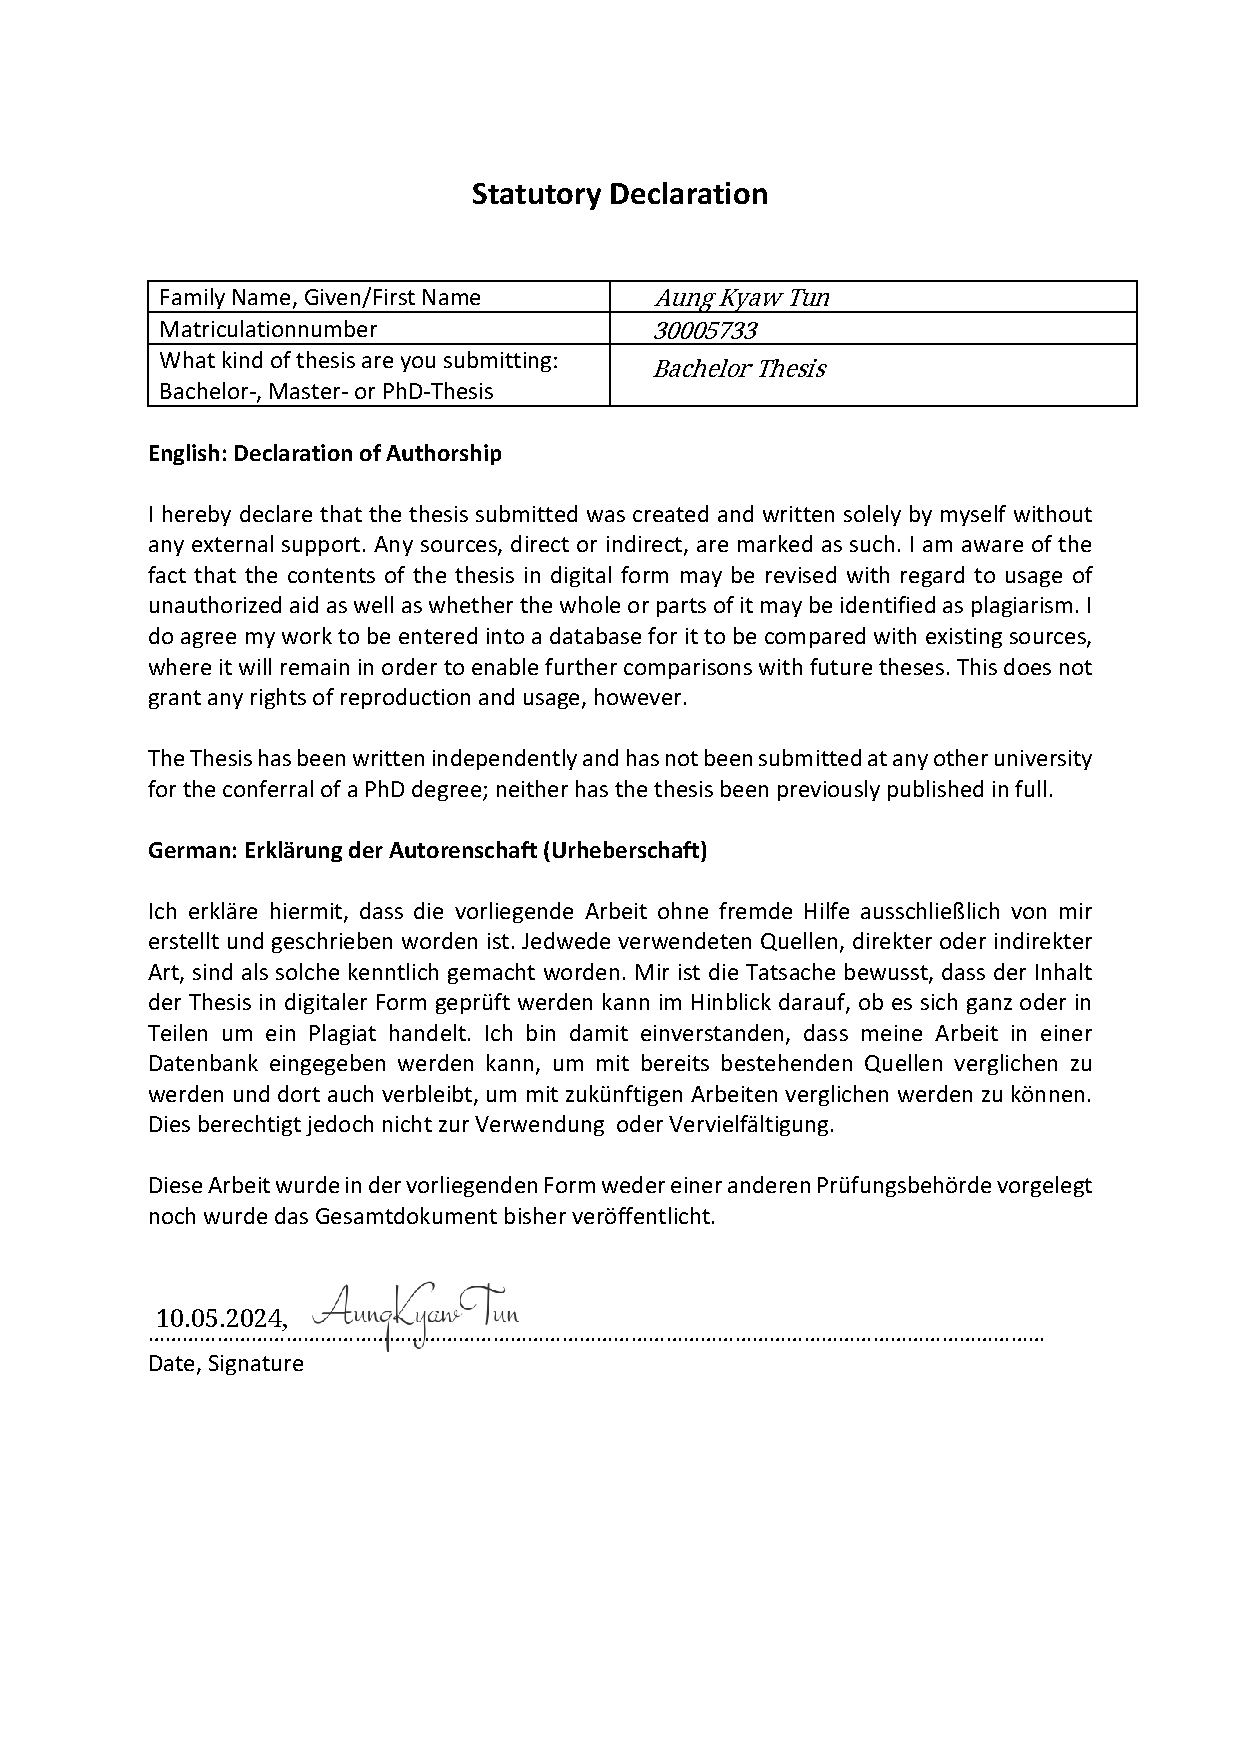
\includepdf[pages=1]{00_Intro_Pages/declaration.pdf}
%\includegraphics

%\clearpage


% Switch from 03a_Certificate to 03b_Certificate for a fancier format.
%%~~~~~~~~~~~~~~~~~~~~~~~~~~~~~~~~~~~~~~~~~~~~~~~~~~~~~~~~~~~~~~~~~~~~~~~~~~~~~~~~~~~~~~~~~%
%	                                    ACKNOWLEDGEMENT                                   %
%~~~~~~~~~~~~~~~~~~~~~~~~~~~~~~~~~~~~~~~~~~~~~~~~~~~~~~~~~~~~~~~~~~~~~~~~~~~~~~~~~~~~~~~~~%
\begin{center}
{\large{\bf{ACKNOWLEDGEMENT}}}
\end{center}
%\thispagestyle{empty}


\noindent
[\textit{Sample:}] I thank everyone who has assisted me in seeing this project through to its completion. I would like to first express my profound gratitude and deepest regards to [Project Guide(s)], IISER Thiruvananthapuram, and sincerely wish to acknowledge [his/her/their] vision, guidance, valuable feedback and constant support throughout the duration of this project.

I am indebted to [Insert Names] for their steadfast encouragement and time. I am lastly grateful to the Indian Institute of Science Education and Research Thiruvananthapuram for providing the necessary resources and facilities to complete this project to the best of my ability.

% Use words like "hard work", "helping every step of the way", 
% "sincere gratitude", "deepest appreciation", "highly indebted",
% "considerate endorsement", "honest and cooperative response", "pivotal care and well wishes"
% "constant support, utmost patience and trust with respect to this project"
% "intuitiveness and insight have been invaluable to the progression of this project, allowing it to mature into the project it is today."
% "valuable guidance kept the project afloat, especially with [his/her/their] fresh take with every stage of development for this project."

\vspace{4cm} % Reduce if text overflows to a new page

\noindent Thiruvananthapuram - 695 551 \hfill \textbf{[Full Name]}

\noindent \today \hfill

\clearpage
%~~~~~~~~~~~~~~~~~~~~~~~~~~~~~~~~~~~~~~~~~~~~~~~~~~~~~~~~~~~~~~~~~~~~~~~~~~~~~~~~~~~~~~~~~%
%	                                     ABSTRACT   	                                  %
%~~~~~~~~~~~~~~~~~~~~~~~~~~~~~~~~~~~~~~~~~~~~~~~~~~~~~~~~~~~~~~~~~~~~~~~~~~~~~~~~~~~~~~~~~%
\vspace{0.5pt}
\begin{flushleft}
    \setlength{\parskip}{0pt}
        %\bigskip
    {\raggedright{{\Large{\bf{ABSTRACT}}}} \par}
    \bigskip
    \vspace{6pt}
    

\end{flushleft} % This section is not essential for the abstract

As autonomous vehicles are entering the market more rapidly with advancements in Machine Learning and Computer Vision, it becomes a necessity to develop a robust algorithm that allows the vehicles to predict the trajectory motion of their nearby objects. One such established algorithm, comparable to the state-of-the-art method, is (Enhanced) Graph-based Interaction-aware Trajectory Prediction(GRIP++). The algorithm uses Gated Recurrent Units (GRU) and Long Short-term Memory (LSTM) type of Recurrent Neural Network(RNN) to train the model with the ApolloScape 3D Trajectory dataset. This paper studies the algorithm in detail, implements object detection and semantic segmentation, and evaluates the results using the Joint Attention in Autonomous Driving (JAAD) dataset, which provides data on pedestrian behavior in traffic scenarios.

\vspace{3cm} % Reduce if text overflowing to a new page. Don't make it too long.

\raggedright{{\large \textbf{Keywords: }}}\par{\large Motion Prediction, Trajectory Prediction, Computer Vision, Machine Learning, Deep Learning, Long short-term memory, Recurrent neural networks, Graph-based motion prediction}
\vfill
\clearpage
%~~~~~~~~~~~~~~~~~~~~~~~~~~~~~~~~~~~~~~~~~~~~~~~~~~~~~~~~~~~~~~~~~~~~~~~~~~~~~~~~~~~~~~~~~%
%                   TABLE OF CONTENTS, LIST OF FIGURES, LIST OF TABLES                    %
%~~~~~~~~~~~~~~~~~~~~~~~~~~~~~~~~~~~~~~~~~~~~~~~~~~~~~~~~~~~~~~~~~~~~~~~~~~~~~~~~~~~~~~~~~%

\tableofcontents
\clearpage
%\listoffigures
%\listoftables

\newpage
%%~~~~~~~~~~~~~~~~~~~~~~~~~~~~~~~~~~~~~~~~~~~~~~~~~~~~~~~~~~~~~~~~~~~~~~~~~~~~~~~~~~~~~~~~~%
%                               NOTATIONS AND ABBREVIATIONS                               %
%~~~~~~~~~~~~~~~~~~~~~~~~~~~~~~~~~~~~~~~~~~~~~~~~~~~~~~~~~~~~~~~~~~~~~~~~~~~~~~~~~~~~~~~~~%
% NOTE: YOU WILL NEED TO ENABLE LINES 115-125 of report.tex OR
%       MAKE USE OF THE listsofsymbols PACKAGE

% The listof___ inputs below are used to generate tables for the symbols,
% constants and nomenclature and take inputs of l, c, r to determine their
% respective column alignments as do any other tables in  LaTeX.

\clearpage % Start a new page

\setstretch{1.5} % Set the line spacing to 1.5, this makes any following tables easier to read.

\noindent

{\Huge{\bf{Notations and Abbreviations}}}\
\\[6pt] 

% NOTE: YOU WILL NEED TO ENABLE LINES 127-137 of report.tex

% sAMPLE OF USE:

%\listofsymbols{ll} % Include a list of Abbreviations (a table of two columns)
%{
%\textbf{FEA} & \textbf{F}inite \textbf{E}lement \textbf{A}nalysis \\
%\textbf{FEM} & \textbf{F}inite \textbf{E}lement \textbf{M}ethod \\
%\textbf{LVDT} & \textbf{L}inear \textbf{V}ariable \textbf{D}ifferential \textbf{T}ransformer \\
%\textbf{RC} & \textbf{R}einforced \textbf{C}oncrete\\
%\textbf{Acronym} & \textbf{W}hat (it) \textbf{S}tands \textbf{F}or \\
%}

No notation is used in this document. No abbreviations have been used either.

\newpage

%~~~~~~~~~~~~~~~~~~~~~~~~~~~~~~~~~~~~~~~~~~~~~~~~~~~~~~~~~~~~~~~~~~~~~~~~~~~~~~~~~~~~~~~~~%
%                                   PHYSICAL CONSTANTS                                    %
%~~~~~~~~~~~~~~~~~~~~~~~~~~~~~~~~~~~~~~~~~~~~~~~~~~~~~~~~~~~~~~~~~~~~~~~~~~~~~~~~~~~~~~~~~%

% % NOTE: YOU WILL NEED TO ENABLE LINES 139-149 of report.tex

%\clearpage % Start a new page

% SAMPLE OF USE:

%{\Huge{\bf{Physical Constants}}}
%\\[6pt]
%\listofconstants{lrcl} % Include a list of Physical Constants (a four-column table)
%{
%Speed of Light & $c$ & $=$ & $2.997\ 924\ 58\times10^{8}\ \mbox{ms}^{-\mbox{s}}$ (exact)\\
% Constant Name & Symbol & = & Constant Value (with units) \\
%}
%\newpage

%~~~~~~~~~~~~~~~~~~~~~~~~~~~~~~~~~~~~~~~~~~~~~~~~~~~~~~~~~~~~~~~~~~~~~~~~~~~~~~~~~~~~~~~~~%
%                                         SYMBOLS                                         %
%~~~~~~~~~~~~~~~~~~~~~~~~~~~~~~~~~~~~~~~~~~~~~~~~~~~~~~~~~~~~~~~~~~~~~~~~~~~~~~~~~~~~~~~~~%

%\clearpage % Start a new page

% SAMPLE OF USE:

%{\Huge{\bf{Symbols}}}
%\\[6pt]
%\listofnomenclature{lll} % Include a list of Symbols (a two-column table)
%{
%$D^{el}$ & elasticity tensor \\
%$\sigma$ & stress tensor \\
%$ \varepsilon $ & strain tensor \\
% Symbol & Name & Unit \\
%}
%\newpage

\pagenumbering{arabic}
\setcounter{page}{1}

%~~~~~~~~~~~~~~~~~~~~~~~~~~~~~~~ Main chapters start here ~~~~~~~~~~~~~~~~~~~~~~~~~~~~~~~~%

\chapter{Introduction} 

\tab Development in the area of Artificial Intelligence, Machine Learning, and Computer vision has been surging in the recent couple of years \cite{8793868}. With it, autonomous vehicles are becoming more available commercially \cite{2019itsc_grip}.  Despite advancement in the field, mass production of self-driving cars and their deployment in everyday life would be only possible if their safety is verified \cite{9756903}. This poses a challenge, especially due to the reported traffic incidents in 2018 from leading companies in the area such as Tesla and Uber \cite{2019itsc_grip}, and has caused concern for the safety of autonomous vehicles (AV). 

\tab One of the aspects that need to be improved in order to ensure the safety of AV is predicting the future positions of the surrounding close-by objects \cite{9756903} just like in the case of human drivers. It is argued that if AV are to predict the future locations of the nearby traffic participants precisely, traffic accidents can be avoided \cite{2019itsc_grip}. Therefore, to ensure their safety, it is imperative to improve the performance of the algorithms used in AV for trajectory prediction.

\tab Various algorithms have been developed to that effect, with numerous car manufacturers working towards improving vehicle safety via better designs of Advanced Driver-Assistance Systems (ADAS) \cite{8793868}. However, much needs to be done in the area. Developing technologies for self-driving cars is also not a recent phenomenon. We can trace its development back to as early as the 1980s \cite{8793868}, especially with Dean A. Pomerleau's work on ALVINN in 1989 that utilized neural networks for the purpose of autonomous navigation \cite{Pomerleau-1989-15721}. These early advancements helped us reach where we currently stand today, which offers different algorithms and models tailored for trajectory prediction that deploy different techniques such as the Kalman Filter, Hidden Markov Model, Bayesian Networks, Gaussian Processes, or using Machine Learning models with Convolutional Neural Network (CNN) and Recurrent Neural Network(RNN); more specifically Long Short-Term Memory(LSTM), Gated Recurrent Unit (GRU), Conditional Variational Auto-Encoder (CVAE), etc. \cite{8793868}.

\tab The focus of this paper is on one particular scheme, developed by Li et al. \cite{li2020gripplus}, called (Enhanced) Graph-based Interaction-aware Trajectory Prediction (GRIP++) that uses graph convolutions to extract features and applies LSTM to make predictions. In this research, the GRIP++ algorithm was analyzed and applied to the JAAD dataset \cite{rasouli2017ICCVW} focused on pedestrian behavior in traffic scenarios. To enhance the analysis, object detection was performed using YOLO \cite{yolov3}, identifying traffic agents like pedestrians and vehicles. Additionally, semantic segmentation was applied to the video data using DeepLabV3+ \cite{DBLP:journals/corr/abs-1802-02611}, which allowed for the identification of drivable areas, crosswalks, and other relevant scene elements. The predicted trajectories, obtained after training and testing the GRIP++ model, were then overlaid onto the processed video, providing visualization of how well the model predicts pedestrian movement in a given traffic scene.






% Remember to input this to the presentative tex file before compiling.
\chapter{Related Work}

\tab There exists a number of challenges in predicting trajectories in the context of self-driving cars. One of those crucial factors is behavior of pedestrians. Due to their ability to move around freely and cross the streets in the same environment as AV, it is important that their safety is ensured by the self-driving cars, irrespective of pedestrians' actions \cite{fragkedaki2024pedestrianmotionpredictionusing}. Because of their "large degree of freedom" \cite{fragkedaki2024pedestrianmotionpredictionusing}, it becomes challenging to model their behavior in a dataset. Therefore other largely available datasets don't provide information for autonomous cars to understand the intention of other traffic agents \cite{rasouli2017ICCVW}. Studies, such as those by Rasouli et al.\cite{rasouli2017ICCVW}, emphasize that pedestrians often engage in non-verbal communication, such as eye contact or gestures, which can significantly influence traffic flow and the decisions made by AV systems. To this end, in their paper "Are they going to Cross?" \cite{rasouli2017ICCVW}, Rasouli et al. introduced a new dataset, Joint Attention in Autonomous Driving (JAAD), which provides not only bounding box information for object detection, but also is annotated with behaviour and contextual details of those present in the traffic scenes. Figure \ref{fig:jaad1} gives an example of the annotations provided by JAAD dataset. 


\begin{figure}[h]
  \begin{center}
     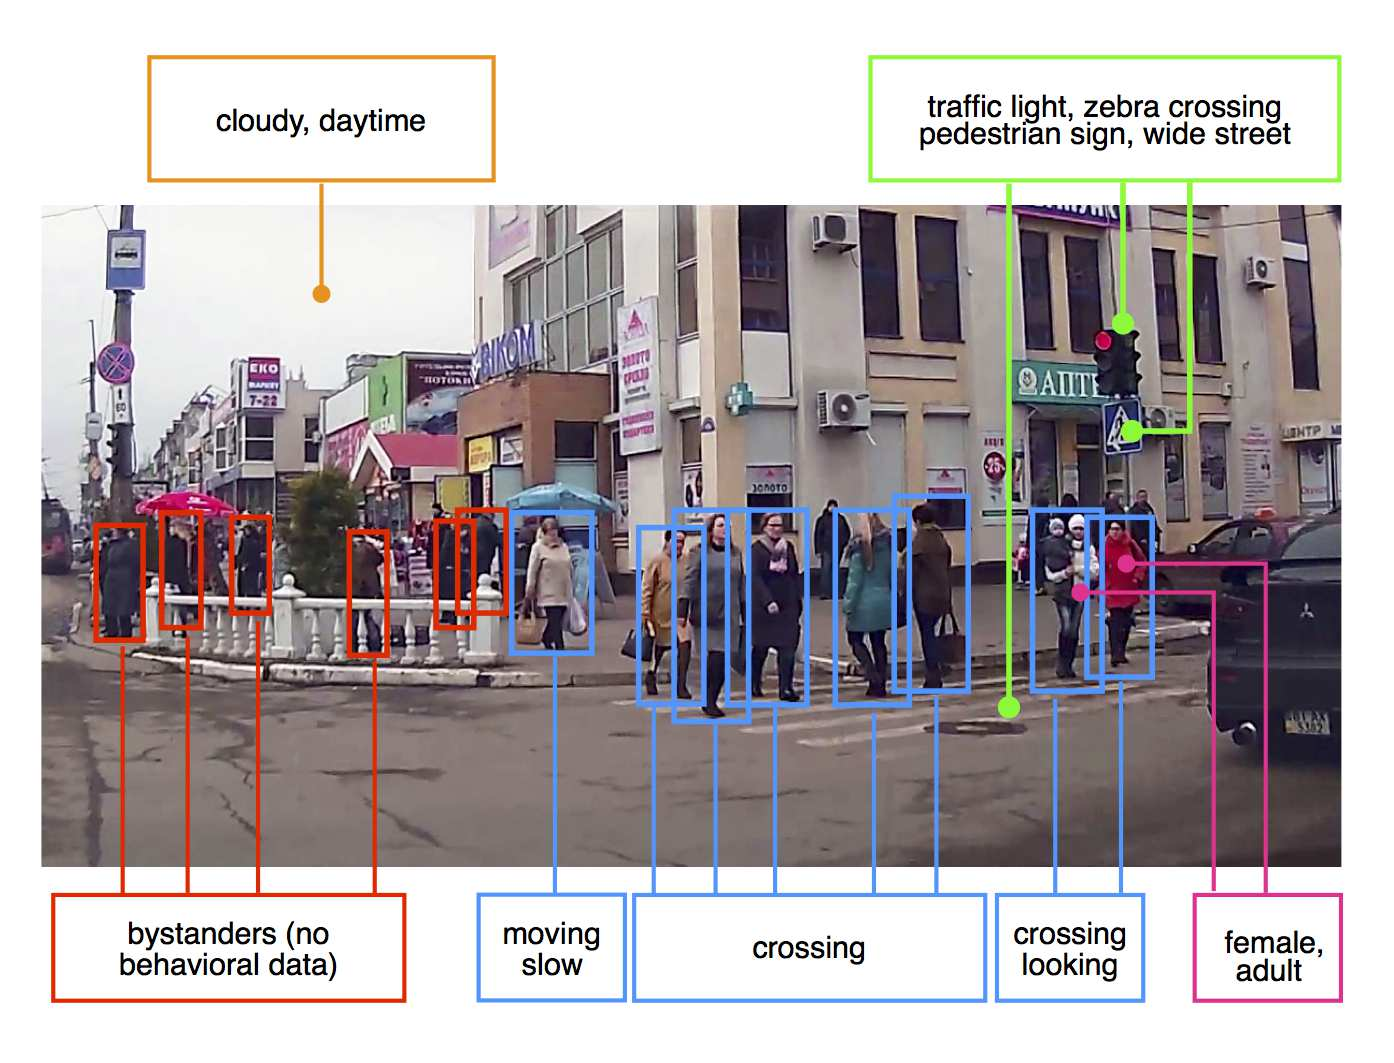
\includegraphics[height=90mm]{Images/Figures/jaad_fig1.png}
  \end{center}
  \caption{JAAD annotations with bounding boxes for all pedestrians, behavioral labels and contextual tags}
  \label{fig:jaad1}
\end{figure}

\tab JAAD dataset particularly focuses on numerous crossing scenarios for pedestrians as the authors of the paper consider most of the interaction with the driving cars to happen at the crossing points \cite{rasouli2017ICCVW}. Their dataset includes three types of ground truth annotations: bounding boxes of pedestrians for object detection, behavioral tags for denoting pedestrians' states and scene annotations for environmental contextual elements. The behavioral information includes the type and duration of pedestrians' actions, as well as the actions of the driver. Pedestrians' actions are divided into three categories: Precondition - pedestrians' state before crossing (i.e., standing, moving slowly, or fast), Attention - pedestrians' awareness towards approaching vehicle , looking for more than 1 second or glancing for less than 1 second, and Response - actions of the pedestrians after being aware of the approaching vehicle. This includes responses such as stopping, clearing the path, slowing down, speeding up, hand gestures, or nodding in reaction to the vehicle. Additionally, complementary tags come with demographics of the pedestrians like gender, age (adult, child, elderly), and group size.
Figure \ref{fig:jaad2} describes an example of behavioral labelling. 


\begin{figure}[h]
  \begin{center}
     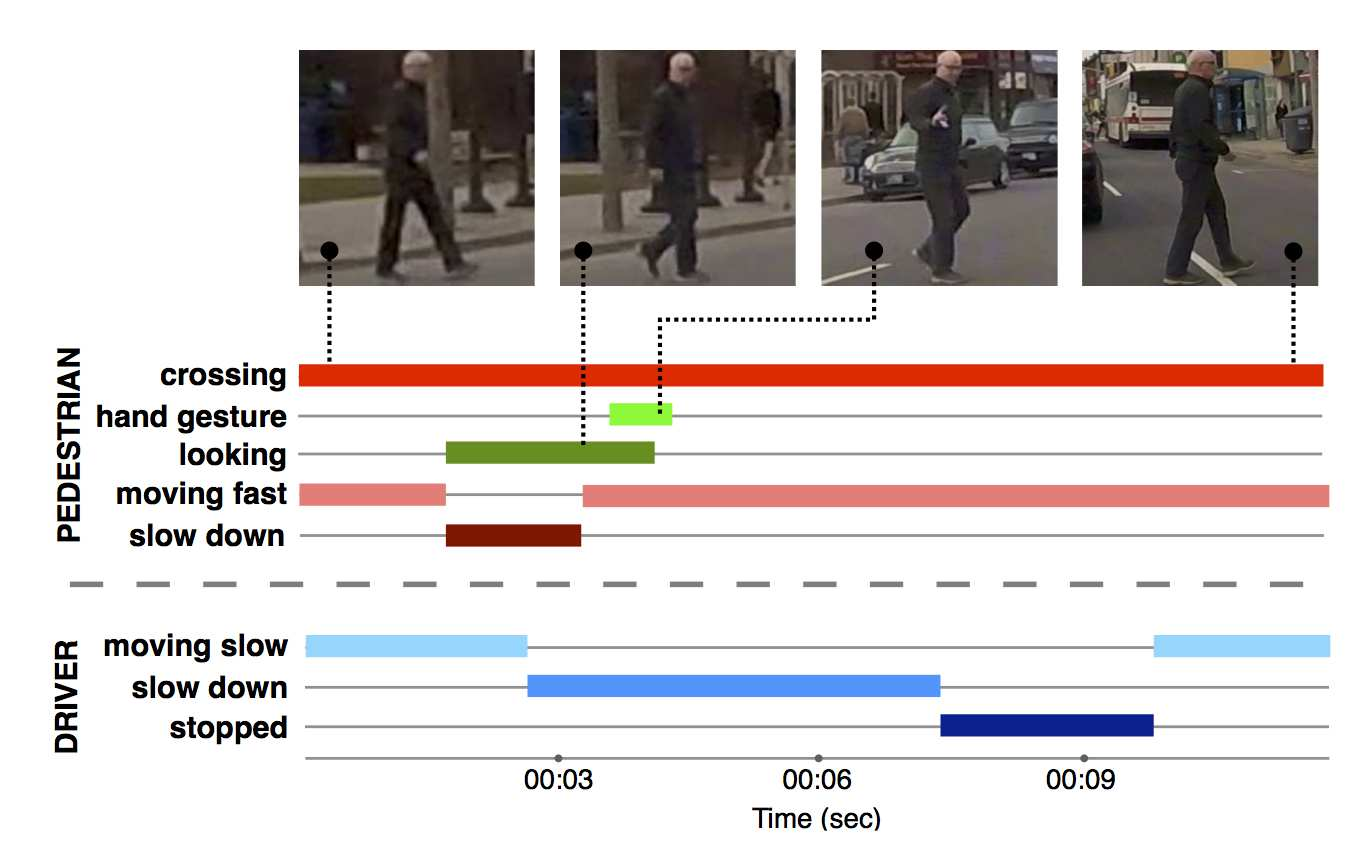
\includegraphics[height=90mm]{Images/Figures/jaad_fig2.png}
  \end{center}
  \caption{JAAD behavioral annotations with timestamps at a crossing point}
  \label{fig:jaad2}
\end{figure}

\tab Another crucial factor in AV system and subsequently for trajectory prediction is to get enhanced information about the driving environment, such as crosswalks, sidewalks, drivable areas and other contextually essential features, that is needed to make informed decisions from the side of AV.  The segmentation process assigns semantic labels to each pixel in an image, distinguishing between different object types and scene elements \cite{sun2024semanticformerholisticsemantictraffic}. Semantics segmentation helps to improve the safety of AV's operation by outlining drivable area and lane markings \cite{che2024twinlitenetplusstrongermodelrealtime}. Deep neural networks employ encoder-decoder structures or spatial pyramid pooling modules to perform semantic segmentation tasks \cite{DBLP:journals/corr/abs-1802-02611}. Encoder-decoder capture sharper object boundaries and gradually recovers the spatial information whereas spatial pyramid pooling encodes multi-scale contextual information by probing the incoming features with filters or pooling operations at multiple rates and multiple effective fields-of-view \cite{DBLP:journals/corr/abs-1802-02611}. DeepLabV3+ \cite{DBLP:journals/corr/abs-1802-02611} combines both these methods that allows them to achieve refined segmentation results along object boundaries. Figure \ref{fig:deeplab} shows the application of DeepLabV3+ on Cityscapes dataset.


\begin{figure}[h]
  \begin{center}
     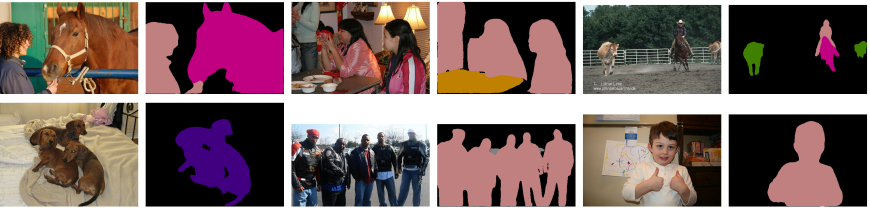
\includegraphics[scale=0.5]{Images/Figures/deeplabv3+.png}
  \end{center}
  \caption{Semantics Segmentation of DeepLabV3+ on Cityscapes dataset}
  \label{fig:deeplab}
\end{figure}

\tab Yet another component required in an AV system is object detection. This process involves locating and categorizing objects \cite{silva2024recurrentyolov8basedframeworkeventbased} within an image or a video frame. Development in the field has been made commonly with the use of Deep learning algorithms such as You Only Look Once (YOLO) detectors that is based on Convolutional Neural Network(CNN) \cite{silva2024recurrentyolov8basedframeworkeventbased}. YOLO is able to perform object detection in real-time, with a fast speed and great accuracy \cite{yolov3}. For this reason, YOLO was later applied on the dataset for safe navigation of autonomous vehicles in a traffic scene.

\tab Although a lot is being done for trajectory prediction on objects, only a number of them consider the importance of nearby objects \cite{2019itsc_grip}. This issue has been taken into consideration and new researches have been made that takes into account the "social interaction" \cite{10397282} between target vehicle, that which we want to predict the trajectory, and its environment that contains other traffic agents such as bicycles, cars and pedestrians. 



\tab Cui et al. \cite{8793868} proposed, focusing on multi-modality of a traffic scenario, a method to predict multiple possible trajectories of a given actor as well as estimating their probabilities. Their proposed network encodes  \(300 \times 300\) bird-eye-view raster image of a nearby traffic actor with \(0.2m\) resolution and the actor's current state, such as velocity, acceleration, heading change rate, as input and outputs \(M\) modes of future \(x-\) and \(y-\) positions. The positions are outputted with \(2H\) per mode, where \(H\) denotes the number of future consecutive time steps for which the states are predicted along with their probabilities. This overall results in \((2H + 1)M\) outputs for each actor. To ensure that the probability outputs sum up to 1, they pass the results through a softmax layer. Their method allows any CNN architecture to be used as the base network and the authors applied MobileNet-v2. 

\tab Luo et al. \cite{luo2020fastfuriousrealtime} introduced in their paper a fast detection, tracking and motion predicting of objects. Bird's eye view LiDAR data is given as input and 3D is processed spatially and temporally. Afterwards they add two branches of convolutional layers where one calculates the probability of a vehicle being at a given location and the other forecasts bounding boxes of the subsequent frames. These available approaches require high computational power if they are to perform trajectory predictions of all nearby objects in a traffic scene \cite{2019itsc_grip}. Therefore Li et al. developed a robust and more efficient object trajectory prediction scheme to forecast the accurate future positions of those objects surrounding the self-driving cars \cite{2019itsc_grip}. Moreover they further improved  their scheme \cite{li2020gripplus} and this paper utilizes the enhanced version.


\section{GRIP Scheme Description}

\tab The algorithm that will be the focus of this paper is Enhanced Graph-based Interaction-aware Trajectory Prediction (GRIP++) \cite{li2020gripplus}. It is designed to predict trajectory of traffic participants around an AV more efficiently using graph to represent interaction amongst close objects, applies multiple graph convolutional blocks to extract features and ultimately uses LSTM encoder-decoder to make predictions. This section summarizes and provides a detailed description of the scheme.

\subsection{Analysis}

\tab Most of the algorithms used in the traffic scene are limited in several ways such as one where it doesn’t work in crowded scenarios, or with the second example it merely predicts the trajectory of one specific car but since the traffic will be composed of more than one vehicle at a given time, this method becomes highly inefficient. Nonetheless these methods require intensive computation power if they want to predict the trajectory of all surrounding objects. And if they are maneuver based, wrong classification of the maneuver type will negatively impact the trajectory prediction.

\tab Li et al., formulates the problem as follows: trajectory prediction is a problem that estimates the future positions of all objects in a scene based on their trajectory histories. Therefore the inputs X of the model are trajectory histories(over \(t_h\) time steps) of all observed objects in a traffic scene:

\begin{equation}
    X = [p^{(1)}, p^{(2)},.....,p^{(t_h)}]
\end{equation}

where,

\begin{equation}
    p^{(t)} = [x_0^{(t)}, y_0^{(t)}, x_1^{(t)}, y_1^{(t)}, ... ,x_n^{(t)}, y_n^{(t)}]
\end{equation}


are the coordinates of all observed objects at time t, and n is the number of observed objects in that scenario. Their format is the same as another study done by Deo et al. and global coordinates are used. To improve the prediction accuracy, the “ego-vehicle-based” coordinate system could be used as suggested by the author but is not applied for future work. 
Because their model takes in histories of all observed objects in a traffic scenario, it was argued to be most fitting to predict the future position of all of them simultaneously rather than focusing on one individual object, which is a preferred measure for other schemes that are also predicting future position for autonomous cars. The outputs Y of the proposed model are the predicted positions of all observed objects in a scenario from time step \(t_h + 1\) to \(t_h+ t_f :\)

\begin{equation}
    Y = [p^{(t_h+1)}, p^{(t_h+2)},........., p^{(t_h+t_f)}]
\end{equation}

where \(p^{(t)}\) is the same as the second equation described above and \(t_f\) is the predicted horizon.

\tab In there proposed scheme , the authors of the paper divide their approach towards their novel model into following components: 
\begin{enumerate}
    \item Input Preprocessing Model,
    \item Graph Convolution Model
    \item Trajectory Prediction Model
    \item Implementation Details
\end{enumerate}

\subsubsection{Input Preprocessing Model}

\textbf{\textit{A. Input Representation:}} Prior to feeding the raw data into the model, it is required to convert it into a specific format for subsequent efficient computation. Given \(n\) objects in a traffic scene in the past \(t_h\) time steps, it is represented in a 3D array \(F_{input}\) with a size of \((n \times t_h \times c)\). The authors set \(c= 2\) in the paper to indicate x and y coordinates of an object. Since it is easier to predict the velocity of an object rather than predicting its location(Li et al., 2020), velocities \((p^{t+1} - p^t)\) is calculated before feeding the data into the model. 

\textbf{\textit{B. Graph Construction:}} As in an autonomous driving application scenario, the movement of a target’s surrounding objects deeply impacts the motion of the target, the authors represent the inter-object interaction using an undirected graph \(G= \{V, E\}\). Each node, \(V\) corresponds to an object present in a traffic scene. Given that each object would have different states at different time steps, the node set \(V = \{v_{it}| i=1,....,n, t =1,...t_h\}\) where \(n\) is the number of observed objects and \(t_h\) is the observed time steps. The feature vector \(v_it\) on a node is the coordinate of \(i_{th}\) object at time \(t\).

\tab In constructing the graph, objects that have interaction at each time step \(t\) are connected via edges. Authors define such interaction in an autonomous driving scenario when two objects are close to each other. Therefore the edge set \(E\) consists two parts: (a) the interaction information between two objects in spatial space time \(t\), called “spatial edge” (Li et al., 2020) and denoted as \(E_S = \{v_{it}v_{jt}|(i,j \in D)\}\), with \(D\) being a set where objects are close to each other. This is demonstrated in the Figure \ref{fig:gripscheme}, using two blue circles with a \(D_{close}\) radius on the “Raw Data” section. Objects that are inside the blue circle are regarded as close to the object located in the middle, indicated by a blue dot. Therefore in the diagram, the top object has three close neighbors whereas the one below has one neighbor. (b) The second part is the “inter-frame edges” (Li et al., 2020), that essentially represents the historical information frame by frame in temporal space. The temporal edge connects each observed object in a given time step with itself in another time step, and is denoted as \(E_F = \{v_{it}v_{i(t+1)}\}\). In such a way\(E_F\) contains all edges of a particular object which represent its trajectory over time steps. 

\tab The authors of the algorithm represent this graph using an adjacency matrix \(A = \{A_0, A_1\}\),  where \(A_0\), an identity matrix \(I\), represents self-connections and \(A_1\), an adjacency matrix, represents spatial connection, for more efficient computation. At a given time \(t\),


\begin{equation}
    A_0[i][j] (or A_1[i][j]) = 
    \begin{cases}
        1, & \text{if edge} {0.5mm} \langle v_{it}, v_{jt}\rangle  \in E\\
        0, & \text{otherwise}
    \end{cases}
\end{equation}

\(A_0\) and \(A_1\) both are of size (\(n \times n\)), where \(n\) is the number of observed objects in a traffic scene. The authors called it “Fixed Graph” as  it is constructed on a manual design rule and is fixed once the input data is given and will not modify during the training phase. It is shown in Figure \ref{fig:gripscheme} as a blue dots connected graph symbol. 

\begin{figure}[h]
  \begin{center}
     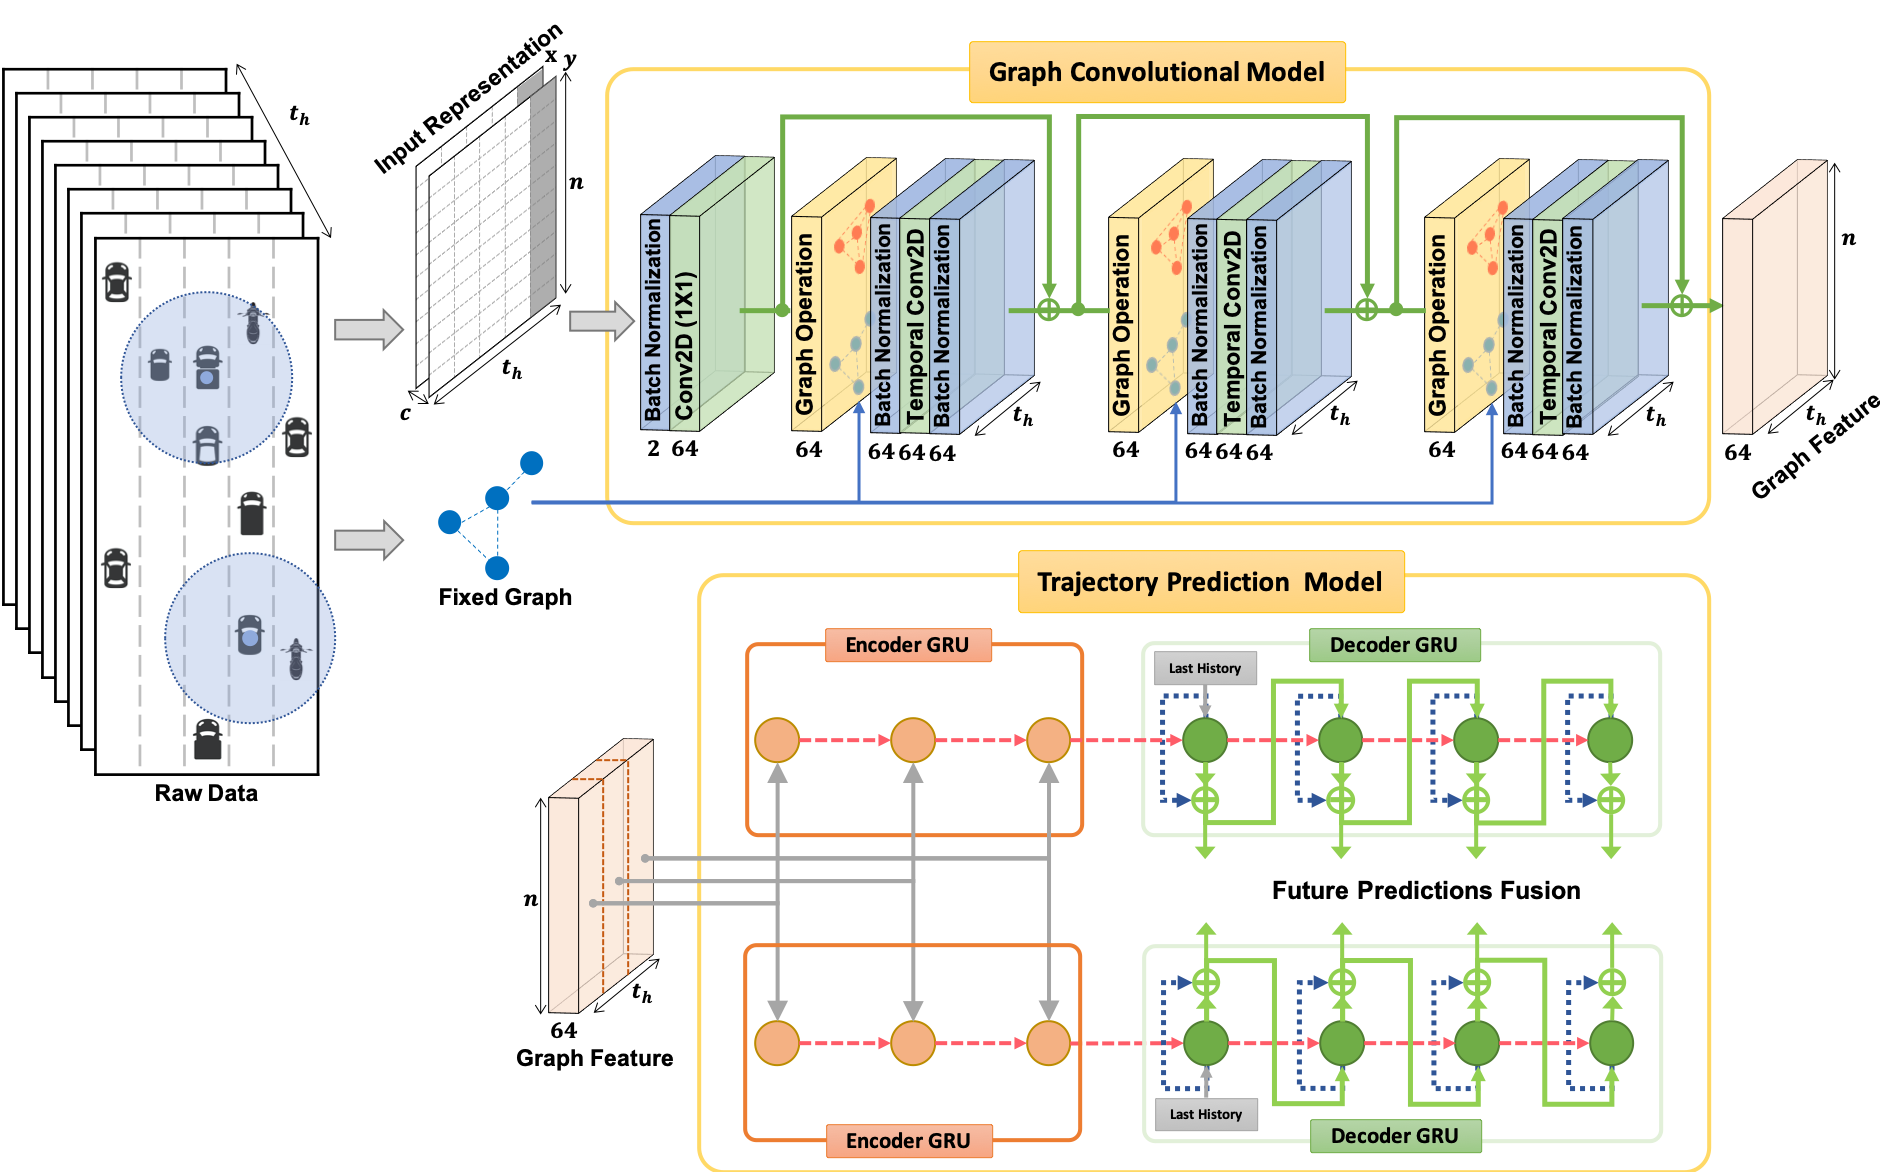
\includegraphics[height=90mm]{Images/Figures/figure1.png}
  \end{center}
  \caption{GRIP++ proposed Scheme}
  \label{fig:gripscheme}
\end{figure}

\subsubsection{Graph Convolutional Model}

\tab For a given preprocessed input data \(F_{input} := \mathbb{R}^{n \times t_h \times c}\), the Graph Convolutional Model passes it through a 2D convolutional layer with \((1 \times 1)\) kernel size, shown in Figure \ref{fig:gripscheme} as "Conv2D \((1 \times 1)\)", so that the number of channel is increased. It is designed to map the 2 dimensional input data (x and y coordinates) into a higher dimensional space to help the model learn a good representation for the trajectory prediction task. The output, therefore, is of the shape \((n \times t_h \times C)\), where \(C\) is the new number of channels. In the figure \ref{fig:gripscheme}, \(C\) is 64. The input data is then fed into both several graph operations and temporal convolutions where graph operations handle the inter-object interaction in spatial space and temporal convolutions capture useful temporal features such as motion pattern of an object. Therefore, Figure \ref{fig:gripscheme}, with 3 Graph Operation layers and 3 Temporal Convolution layers shown, one Temporal Convolution layer is added at the end of each Graph Operation layer to process the input data both spatially and temporally in every alternate. 

\tab Batch Normalization layers are added as well to improve the stability of the model in training. Skip connections, denoted as green polylines, are used to ascertain that the model can propagate larger gradients to initial layers, which could learn as fast as the final layers.

\textbf{\textit{1) Graph Operation Layer:}} A graph operation layer takes into account the interactions of surrounding objects. There are two graphs in each Graph Operation layer: (i) a Fixed Graph, which is the adjacency matrix \(A\) shown above and the blue graph symbol from Figure \ref{fig:gripscheme}, constructed based on the current input, and (ii) a trainable graph, \(G_{train}\), shown in Figure \ref{fig:gripscheme} as orange graph symbol in the Graph Operation Model block.

\tab The authors normalize the Fixed Graph A using the below equation to make sure that the value range of feature maps are not changed after the graph operations: 

\begin{equation}
    G^j_{fixed} = \Lambda^{-1/2}_j A_j \Lambda^{-1/2}_j
\end{equation}

where \(\Lambda^{-1/2}_j\) is computed as:

\begin{equation}
    \Lambda^{ii}_j = \sum_k (A^{ik}_j) + \alpha
\end{equation}

\(\alpha\) is set to \(0.001\) to avoid empty rows in \(A_j\).

\tab Since the Fixed Graph, \(G_{fixed}\) is constructed based on a manually designed rule, it might not be able to represent the interactions of objects properly. Therefore to solve this problem, the authors of the paper sum the Fixed Graph with the trainable graph so that the trainable graph can be trained to overcome this limitation. As a result, after a Graph Operation layer takes an input \(f_{conv}\) from the previous layer, the output feature map \(f_{graph}\) is calculated as: 

\begin{equation}
    f_{graph} = \sum_{j=0}^1(G^j_{fixed} + G^j_{train})f_{conv}
\end{equation}

As the Graph Operation layers do not change the size of the features, \(f_{graph}\) is of size \((n \times t_h \times C)\). 

\textbf{\textit{2) Temporal Convolutional Layer:}} The generated feature \(f_{graph} := \mathbb{R}^{n \times t_h \times C}\) is then fed into a Temporal Convolutional layer. The kernel size of a Temporal layer is set to \((1 \times 3)\) to force the processing of the data along the temporal dimension. Paddings and strides are added appropriately to make sure each layer has an output feature map of expected size. 

\subsubsection{Trajectory Prediction Model}

\tab This model consists of several networks which share the same Seq2Seq structure but is trained for different weights. Two Seq2Seq networks are shown in Figure \ref{fig:gripscheme}. The Graph Feature, generated by the Graph Convolutional Model, is taken by each network as its input. At each temporal dimension, feature vectors of the Graph Feature are fed into the corresponding input cell of the Encoder GRU (Gated Recurrent Unit). Thereafter the hidden feature of the Encoder GRU together with the coordinates of the objects are fed into the Decoder GRU to predict the position coordinates at the current time step. The input of the first decoding step is the coordinates of objects at the "Last History" step, and the output of the current step is then fed into the next GRU cell. This is illustrated in Figure \ref{fig:gripscheme} as the gray "Last History" boxes corresponding to the gray column of the Input Representation. Above described decoding process is to be repeated multiple times until the positions for all expected time steps \((t_f))\) in the future is predicted by the model. Due to velocity of the traffic agents in a given scene not being constant, the authors have incorporated the model to predict the velocity change by adding a residual connection, shown as blue dashed lines in the Figure \ref{fig:gripscheme}, in between the input and the output of each cell of the Decoder GRU. 

\tab After getting the predicted results of the Seq2Seq networks, the predicted velocities results are averaged at each time step. After averaging the predicted velocities \((\Delta x, \Delta y)\), they are added back to the last historical location \((p^{(th)})\) to convert the predicted results back to \((x, y)\) coordinates. The main difference between implementation of the algorithms GRIP++ and GRIP are listed down as follow:

\begin{itemize}
    \item GRIP++ takes velocity \((\Delta x, \Delta y)\) as input whereas GRIP takes \((x, y)\) coordinates as input
    \item GRIP++ considers both fixed as well as trainable graphs meanwhile GRIP only considers fixed graphs in the graph convolution sub-module
    \item In the graph convolution model GRIP++ uses 3 blocks, adds batch normalization and uses skip connections while GRIP uses 10 blocks without the batch normalization layers.
    \item GRIP++ uses GRU networks, three encoder-decoder blocks for trajectory prediction, and average the results whereas GRIP uses LSTM networks and only one encoder-decoder block for trajectory prediction. 
\end{itemize}


\subsubsection{Implementation Details}

\tab The authors implement the scheme using Python Programming Language and PyTorch Library. This section further details the implementation of the scheme and the settings of necessary parameters.

\tab \textbf{Input Preprocessing Model:} The authors propose, in their paper, a traffic scene within 180 feet (\(\pm 90\) feet), whereby all the objects within the designated region will be observed and predicted in the future. Furthermore, two objects in a scene are defined as \textit{close} if their distance is less than 25 feet \((D_{close} = 25)\) and are connected via a spatial edge, \(e_s \in E_S\). 

\tab \textbf{Graph Convolutional Model:} As described above with Figure \ref{fig:gripscheme}, the authors utilize a \((1 \times 1)\) convolutional layer to increase the channel of data input to 64, their Graph Convolutional Model contains 3 Graph Operation layers and each layer is followed by a Temporal Convolution layer that has a convolutional kernel of size \(1 \times 3\). \(stride\) is set to 1 and paddings are added appropriately to maintain the feature maps shape. Therefore, the Graph Convolutional Model outputs a size of \((n \times t_h \times 64)\). Additionally, the scheme dropouts features (0.5 probability) after each graph operation to avoid overfitting. 

\tab \textbf{Trajectory Prediction Model:} The encoder and decoder of this model are both a two-layer GRU networks. The number of hidden units of the two GRUs are set to \(r\) times of the output dimension, \(r \times 2 \times n\), where \(r\) is to improve the representation ability, \(n\) is the number of objects and 2 is the \(x,y\) coordinates. For this paper, the authors choose \(r=30\) for best performance. The 64 channels input of the encoder are the same as the Graph Convolutional Model output.

\tab \textbf{Optimization:} The model is trained as a regression task at each time and the overall lose is computes as:

\begin{equation}
    Loss =  \dfrac{1}{t_f} \sum_{t=1}^{t_f} loss^t
\end{equation}

\begin{equation}
          \tab = \dfrac{1}{t_f} \sum_{t=1}^{t_f} \lVert {Y_{pred}^t - Y_{GT}^t} \rVert
\end{equation}

where \(t_f\) is the time step in the future, which is set to \(4\) in Figure \ref{fig:gripscheme}, \(loss^t\) is the loss at time \(t\), \(Y_{pred}\) and \(Y_{GT}\) are predicted positions and ground truth respectively. And the model is trained such that the \(Loss\) is minimized. 

\tab \textbf{Training Process:} The authors train the model using Adam Optimizer with default settings unchanged in PyTorch Library, with \(batch\_size\) set to \(64\) during training.


\section{Objective}

\tab For this research, primary objective is to answer the following research question: How can the integration of the GRIP++ algorithm with real-time object detection (YOLO) and semantic segmentation (DeepLabv3+) enhance the accuracy of pedestrian trajectory prediction in a self-driving cars context in urban environments?
% Remember to input this to the presentative tex file before compiling.
\chapter{Predicting Pedestrian Trajectories in Driving Environment}

\tab The previous chapter presented an in-depth description and an analysis of the GRIP++ algorithm \cite{li2020gripplus}, explaining its architecture, theoretical foundations, and advantages in predicting trajectories within dynamic traffic environments. To further assess the performance and applicability of GRIP++, the algorithm was implemented on a different dataset from ApolloScape Trajectory dataset \cite{ma2019trafficpredict}, the one originally used by the developers of the algorithm. Instead Joint Attention in Autonomous Driving, (JAAD) \cite{rasouli2017ICCVW} dataset was opted for this operation. JAAD provides extensive examination of joint attention in the autonomous driving context \cite{rasouli2017ICCVW}. The dataset focuses on the behaviour of pedestrians and drivers in a traffic scenario, specifically at the crossing points as well as the factors influencing them. Due to its comprehensive set of annotated videos, it makes it well-suited for the task of predicting pedestrian trajectories and investigating the essential question "Are they going to corss?" \cite{rasouli2017ICCVW}. 

\tab As such this chapter focuses on conversion of JAAD dataset to suitable format, training and testing the dataset to receive predicted trajectory results, which was then incorporated with \verb|YOLO| \cite{yolov3} for object detection and DeepLabV3+ \cite{DBLP:journals/corr/abs-1802-02611} for semantics segmentation to enhance overall accuracy and context-awareness of the predictions. Figure \ref{fig:pipeline} demonstrates the pipeline of this research.

\begin{figure}[h]
  \begin{center}
     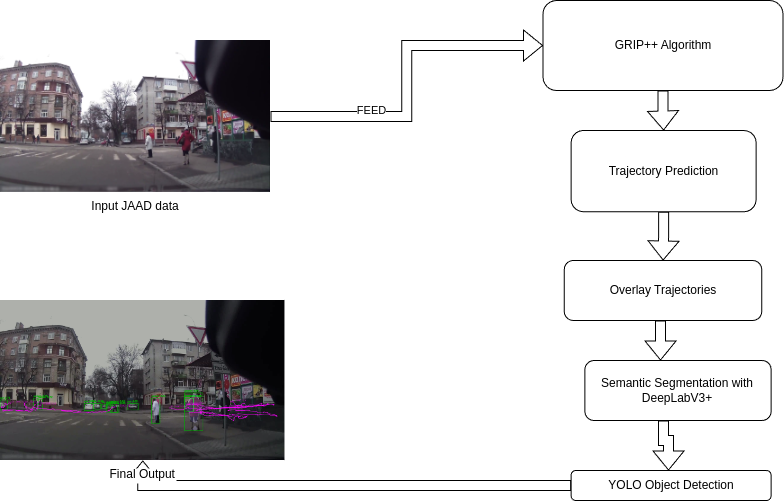
\includegraphics[scale=0.5]{Images/Figures/Pipeline.png}
  \end{center}
  \caption{Pipeline for predicting trajectory in a dynamic driving context}
  \label{fig:pipeline}
\end{figure}

\section{JAAD Dataset}

\tab As briefly mentioned above JAAD provides annotation of a collection of dataset, specially \(346\) short video clips of driving footage, is available to the public for research in autonomous vehicle area. These clips, recorded from various regions of North America and Eastern Europe, capture a variety of common scenes typical of everyday urban driving in a range of weather conditions \cite{rasouli2017ICCVW}. 

\subsection{Annotation Structure of JAAD}

\tab The annotations of JAAD videos are based on the video clip titles. Three kinds of labels are available from JAAD: "pedestrians" (individuals with behavior annotations), "peds" (bystanders who are distant and do not interact with the driver), and "people" (groups of pedestrians) \cite{rasouli2017ICCVW}. The format of each pedestrian's unique id is \verb|0_<video_id>_<pedestrian_number>|. Pedestrians with behavior annotation, have "b" attached at the end of their ids, e.g., \verb|0_1_3b|. Similarly, annotations for people follow the same strucutre but their ids end in the letter "p," such as \verb|0_5_2p|, the annotations for people likewise follow the same structure. For the purpose of using this dataset annotation, however, strings and chars like \verb|"_"|, \verb|"p"|, and \verb|"b"| were removed from the annotations during the \textbf{data transformation} stage since the data structure of the GRIP++ algorithm does not allow for strings to be included in the dataset while preprocessing \cite{ma2019trafficpredict}.

\tab In the annotations, bounding boxes are provided together with occlusion tags for all pedestrians which make the dataset suitable for pedestrian detection. Bounding boxes in each annotation have two coordinate points: the top-left and bottom-right corners, specified as \([x_1, y_1, x_2, y_2]\). Additionally, these bounding boxes are labeled with occlusion tags, where 0 indicates no occlusion, 1 represents partial occlusion (more than 25\%), and 2 denotes full occlusion (more than 75\%).

\tab The annotations within the dataset are categorized into five distinct groups, each for a specific purpose:

\begin{itemize}
    \item \textbf{Annotations}: This group encompasses general video metadata such as attributes related to the time of day, weather conditions, and location. Additionally, it includes detailed information on pedestrian activities (e.g., walking, looking) and bounding box coordinates, along with corresponding occlusion statuses. Notably, activity information is only available for a selected subset of pedestrians. These annotations are recorded for each frame and apply to every labeled instance.
    \item \textbf{Attributes}: Focused on pedestrians with behavior annotations, this category provides demographic details and information regarding crossing points and crossing behavior characteristics. These annotations are assigned to individual pedestrians rather than frames and are intended to offer insights into specific pedestrian behaviors in various traffic scenarios.
    \item \textbf{Appearance}: For videos characterized by high visibility, this group offers details on pedestrian appearance, including pose, clothing, and any objects being carried. This information is annotated per frame for each pedestrian, allowing for a thorough analysis of pedestrian visual characteristics.
    \item \textbf{Traffic}: This group contains traffic-related annotations, offering information on the presence of traffic signs, traffic lights, and other traffic control devices within the scene. These annotations are captured on a per-frame basis, ensuring a comprehensive understanding of the traffic environment during the recorded events.
    \item \textbf{Vehicle}: Vehicle-related actions, such as acceleration, deceleration, or rapid movement, are included in this category and these actions are recorded per frame
\end{itemize}

\tab In the application of the GRIP++ algorithm, not all annotation groups are required. The primary focus is on the dataset annotations group "\textbf{Annotations}," which provide the necessary information for the task. The other groups are considered irrelevant to this particular application and are therefore disregarded.

\section{Data Preparation}

\tab The JAAD dataset, originally structured for analyzing pedestrian behavior in traffic scenarios, required transformation to be suitable with the data format required by the GRIP++ algorithm. The JAAD dataset provides annotations in XML format, detailing pedestrian positions, actions, and interactions with traffic elements. However, the GRIP++ algorithm expects data in a specific structure, similar to the Apolloscape dataset, which was used by the GRIP++ authors for their experiments \cite{li2020gripplus}. To adapt the JAAD dataset to be compatible with GRIP++ requirement, data conversion was carried out. 

\subsection{Data Conversion}

\tab The JAAD dataset contains XML annotations for behavior and interactions of pedestrians in urban environments. These XML annotations were first converted into a structured text format that matches the format used by the Apolloscape dataset. Their data structure of each line in the text file is as follow:

\begin{table}[h!]
\centering
\resizebox{\textwidth}{!}{%
\begin{tabular}{|c|c|c|c|c|c|c|c|c|c|}
\hline
frame\_id & object\_id & object\_type & position\_x & position\_y & position\_z & object\_length & object\_width & object\_height & heading \\
\hline
\end{tabular}%
}
\caption{Data Structure of ApolloScape Dataset \cite{ma2019trafficpredict}}
\end{table}

However, since the JAAD dataset does not include information for position\_z, and object\_height, only eight columns were extracted from the JAAD annotations. These columns include frame\_id, object\_id, object\_type, position\_x, position\_y, and heading. The missing columns (i.e. position\_z and object\_height) were omitted because JAAD lacks the necessary 3D positional information and detailed bounding box dimensions available in Apolloscape.

\subsubsection{Heading Calculation}

\tab Although data for "heading" was not readily available, it was computed based on the already accessible information. The heading is an angular measure that represents the orientation or direction of the object with respect to the x-axis \cite{serway2013physics}. For instance, in a traffic scenario, the heading can indicate whether a vehicle is moving forward, turning, or reversing. 
The heading was calculated based on the position of the object’s bounding box. Specifically, the angle of the vector formed by the top-left and bottom-right corners of the bounding box with respect to the x-axis was computed using the \(atan2\) function. This function calculates the arctangent of the two given coordinates, which provides the angular direction of the bounding box in radians. The formula \cite{atan2_cpp_tutorial} used is:

\begin{equation}
    heading = atan2(y_{br} - y_{tl}, x_{br} - x_{tl}) 
\end{equation}

where (x\_{\text{tl}}, y\_{\text{tl}}) is the top-left corner of the bounding box and (x\_{\text{br}}, y\_{\text{br}}) is the bottom-right corner. This heading value was then rounded to three decimal places for consistency. The heading provided directional information that the GRIP++ model could use to better predict future trajectories of moving objects.

\subsubsection{Object Type Mapping}

\tab Each object in the JAAD dataset was assigned a type based on the classification scheme used in the Apolloscape dataset. The object types in Apolloscape include small vehicles, big vehicles, pedestrians, motorcyclists/bicyclists, and others. These types were mapped to corresponding IDs as follows:

\begin{table}[h!]
\centering
\begin{tabular}{|l|c|c|c|c|c|}
\hline
\textbf{Object Type} & \textbf{Small Vehicles} & \textbf{Big Vehicles} & \textbf{Pedestrian} & \textbf{Motorcyclist and Bicyclist} & \textbf{Others} \\
\hline
\text{ID} & 1 & 2 & 3 & 4 & 5 \\
\hline
\end{tabular}
\caption{ApolloScape's object types and their corresponding IDs \cite{ma2019trafficpredict}}
\label{tab:object_type_ids}  % Label for referencing the table
\end{table}


 since the JAAD dataset primarily focuses on pedestrian behavior and interactions, it does not provide detailed information about other types of objects, such as vehicles or bicyclists. As a result, after converting the JAAD dataset into the required format, only two object types are expected to appear in the processed data:

\begin{itemize}
    \item \textbf{Pedestrians} (ID: 3),
    \item \textbf{Others} (ID: 5)
\end{itemize}


The "Others" category contains any objects that are not classified as pedestrians, though in practice, the JAAD dataset contains very few examples outside of the pedestrian category. The object type mapping was still retained to ensure compatibility with the GRIP++ algorithm, which was designed with the Apolloscape dataset's object type distribution in mind.

\subsection{Data Cleaning}

\tab After converting the JAAD dataset into the required format for use with the GRIP++ algorithm, an additional step of data cleaning was performed. This cleaning process was necessary for ensuring that the data was consistent with the expectations of the GRIP++ model and did not introduce unnecessary noise during training and testing. The key steps involved in this process were as follows:

\begin{enumerate}
    \item \textbf{Handling Missing Values}: During the conversion process, some object annotations may have been incomplete or missing entirely. These instances were identified, and any lines or entries with missing values were either corrected or removed to maintain the integrity of the dataset.
    \item \textbf{Filtering Non-Relevant Objects}: As previously noted, the JAAD dataset primarily focuses on pedestrians, with limited information available for other object types such as vehicles. Object types that did not fit into the defined categories of the GRIP++ model were categorized as "Others" (ID: 5), but were still retained in the dataset for completeness.
    \item \textbf{Removing Empty Files}: During the preprocessing stage, some files were found to be empty, meaning they contained no objects or annotations. These empty files were automatically removed from the dataset since such files provided no valuable information for training or testing.
\end{enumerate}

As a result of this data cleaning process, the dataset was reduced from the originally available \(\textbf{346}\) files to \(\textbf{319}\) files. The removed files either contained no annotations or did not meet the necessary criteria for further processing.

\subsection{Data Splitting}

\tab Once the data was transformed and cleaned, it needed to be divided into training and testing sets to train the model and evaluate its performance. For this purpose, the \verb|train_test_split| function from the \verb|scikit-learn| library was used.

Given the original setup by the GRIP++ developers, where a specific ratio of training to testing data was employed, the same principle was adopted in this implementation. The data was split with a ratio of approximately \(55\) to \(1\), following the precedent set by the authors of the GRIP++ algorithm. This ratio was chosen to maintain consistency with their approach and ensure that the training data was sufficiently large while still allowing for adequate evaluation on the test data.


\section{Training and Testing the Model}

\subsection{Model Training SetUp}

\tab The training of the GRIP++ model was conducted on \verb|Google Colab|, which provides access to NVIDIA GPUs, that is required to run the original \verb|Python| file developed by the authors \cite{li2020gripplus}, ensuring the required computational power and CUDA support necessary for training deep learning models. \verb|Colab| was chosen due to its free availability and built-in shared GPU support, making it suitable for models that require intensive computations like GRIP++.

\verb|PyTorch| was used as the primary framework for implementing and training the GRIP++ model. \verb|PyTorch| provides flexibility and ease of use, particularly for graph-based models, which are integral to GRIP++. The CUDA library was leveraged to ensure GPU acceleration, which speeds up matrix operations, tensor computations, and the backpropagation process during training \cite{cuda2024}.

\subsection{Hyperparameters and Configurations}

\tab Several hyperparameters were set for training the GRIP++ model. These include:

\begin{itemize}
    \item \textbf{Learning Rate}: The learning rate was set to an initial value of 0.01. This value was chosen based on experimentation and previous works, balancing between fast convergence and stability of training.
    \item \textbf{Batch Size}: The batch size was set to 64 for training and 32 for validation. This choice balances memory usage and the stability of gradient updates.
    \item \textbf{Number of Epochs}: The training was conducted for 50 epochs. The original paper experimented with various epochs, and similar values were used here to ensure the model converges appropriately.
    \item \textbf{Optimizer}: The Adam optimizer was selected for its adaptive learning rate capabilities, which are particularly beneficial for models like GRIP++ that have complex architectures and large parameter spaces.
\end{itemize}

These configurations were determined based on the original implementation of GRIP++ and fine-tuning through experimentation to optimize performance on the JAAD dataset.

\subsection{Preprocessing and Data Preparation}


\tab Before training, the transformed dataset underwent preprocessing to ensure it was in the correct format for input into the GRIP++ model. This preprocessing involved:

\begin{itemize}
    \item \textbf{Normalizing Position Data}: The positional data (\verb|position_x| and \verb|position_y|) were normalized based on the maximum values in the dataset to prevent issues related to scale during training.
    \item \textbf{Graph Construction}: Each frame in the sequence was represented as a graph, where objects (e.g., pedestrians, vehicles) were nodes, and the edges represented interactions between them. The features associated with each node included the object's type and its spatial information.
    \item \textbf{Sequence Padding}: The sequences were padded to ensure consistent input dimensions for the GRIP++ model, as deep learning models require fixed input sizes. Shorter sequences were padded, while longer sequences were truncated.
\end{itemize}
    

Once preprocessing was complete, the dataset was ready for the training and testing phases.

\subsection{Training Process}

\tab The training process involved the following steps:

\begin{itemize}
    \item \textbf{\textit{Data Loading:}} The preprocessed dataset was loaded using custom data loaders designed to efficiently batch the data for training and testing. This involved dynamically creating batches of data, including the graphs for each frame sequence and the associated labels.
    \item \textbf{\textit{Forward Pass:}} For each batch, the data was passed through the GRIP++ model, where the graph convolutional layers extracted interaction-aware features, and the LSTM layers predicted future trajectories based on these features.
    \item \textbf{\textit{Backpropagation}}: Gradients were computed using backpropagation, and the Adam optimizer was used to update the model's parameters.
    \item \textbf{\textit{Validation}}: After each epoch, the model was evaluated on the validation set to monitor its performance and adjust the learning rate if necessary.
\end{itemize}

\tab This training cycle was repeated for the specified number of epochs, with model checkpoints saved at intervals to prevent data loss and to enable further fine-tuning if required.

\subsection{Challenges}

\tab During the training process, one of the main challenges encountered was the limitations imposed by the available GPU resources on \verb|Google Colab|. While \verb|Colab| provides access to powerful GPUs, there are restrictions on memory usage and the maximum time for continuous usage. These limitations required careful management of the available resources. Training had to be paused or restarted at times, and model checkpoints were regularly saved to avoid data loss.

\section{Results and Analysis}

\subsection{Model Performance Evaluation}

After training the GRIP++ model on the JAAD dataset, the model's performance was evaluated on the test set. The evaluation focused on predicting the future trajectories of pedestrians, as JAAD primarily contains pedestrian data. The predictions were compared against the ground truth to assess the accuracy of the model.

Key performance metrics included:

\begin{itemize}
    \item Average Displacement Error (ADE): Measures the average Euclidean distance between the predicted trajectories and the ground truth over all time steps \cite{ma2019trafficpredict}. This metric is particularly important in trajectory prediction tasks, as it indicates how close the model's predictions are to the actual movement of the objects.
    \item Final Displacement Error (FDE): Evaluates the distance between the predicted final position and the ground truth final position at the last time step \cite{ma2019trafficpredict}. This metric helps assess how well the model predicts the endpoint of a trajectory, which is critical in safety-critical applications like autonomous driving.
\end{itemize}

\begin{table}[ht]
\centering
\begin{tabular*}{\textwidth}{|c@{\extracolsep{\fill}}|c|c|c|}
\hline
\textbf{Method}            & \textbf{Epoch} & \textbf{ADE} & \textbf{FDE} \\
\hline
TrafficPredict             & -              & 7.1811       & 11.121       \\
\hline
GRIP++            & Epoch18             & 0.7142       & 1.3732       \\
\hline
GRIP++ on JAAD     & Epoch21             & 1.66         & 0.15         \\
\hline
GRIP++ on JAAD     & Epoch41             & 12.26        & 0.57         \\
\hline
\end{tabular*}
\caption{Comparison of methods based on ADE and FDE metrics.}
\end{table}



\tab In the first test subset on the JAAD dataset, the GRIP++ model achieved an ADE of 1.66 and an FDE of 0.15. These results indicate that while the model performs reasonably well in predicting pedestrian trajectories overall, it performed exceptionally in final destination prediction, as evidenced by the relatively low FDE. The low FDE suggests that the model's final predictions were close to the actual final positions of pedestrians in the scene. 

The performance on the second test subset was less accurate, with an ADE of 12.26 and an FDE of 0.57, suggesting that in this scenario, the model struggled more with overall trajectory prediction but still performed relatively better in terms of predicting the final position, though less accurately than in the first test.

\subsection{YOLO and DeepLabV3+}

\tab To get an accurate interpretation of the scene, DeepLabv3+ was employed for semantic segmentation. This deep learning model was used to highlight key features in the driving environment, such as drivable areas and crosswalks. By segmenting the scene, it becomes easier to understand the spatial context within which the pedestrians and vehicles are moving. The segmented output identifies safe zones, walkways, and areas that are off-limits, providing a comprehensive view of how pedestrians interact with their environment. This information is particularly valuable when analyzing whether predicted trajectories falls within safe walking paths or if there is a potential risk of crossing into dangerous areas. The integration of semantic segmentation ensures that trajectory predictions are not only accurate but also contextually aware of the environment.

\tab \verb|YOLO| object detection was used to draw bounding boxes around the objects present in the video frames to keep track of the pedestrians' movements and their interaction in real-time. This helped to distinguish pedestrians from other traffic agents and to associate their predicted trajectory with correct individuals. After the semantics segmentation and YOLO application, predicted trajectories were overlaid on the video frames to depict precisely the movements, ids and the anticipated locations of the pedestrians.  

\tab The visualizations showed how the model predicted the next 3 seconds of pedestrian movement. For instance, the model correctly predicted when a pedestrian was likely to stop, move forward, or change direction. This visual validation was essential to verify the model's effectiveness beyond numerical metrics.




\begin{figure}[h]
  \begin{center}
     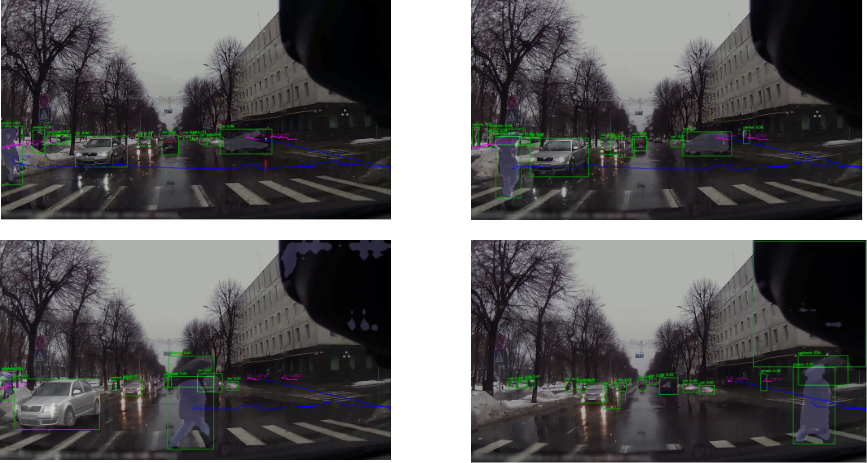
\includegraphics[scale=0.5]{Images/Figures/sequenceofimages.png}
  \end{center}
  \caption{Images from the second test subset}
  \label{fig:testimages}
\end{figure}



\subsection{Qualitative Analysis}

\tab While quantitative metrics like ADE and FDE provide valuable insights, they do not fully capture the complexities of real-world scenarios. One crucial aspect is the inherent uncertainty in pedestrian behavior. Even if the model predicts with 99\% accuracy that a pedestrian will not cross a street, there remains a 1\% chance that they might unexpectedly decide to cross.

\tab This slim margin of uncertainty can have significant consequences. For example, if an autonomous vehicle concludes that a pedestrian is unlikely to cross and continues driving, but the pedestrian suddenly steps into the street, the outcome could be disastrous. Therefore, even models with high predictive accuracy should be used cautiously in critical real-world applications like autonomous driving. Human behavior is unpredictable, and safety systems must account for these rare but potentially catastrophic deviations.

\tab The challenge lies in striking a balance between the model's confidence and the implementation of safety measures that prevent accidents even in rare cases of prediction failure.

\subsection{Challenges and Limitations}


\tab One of the primary challenges encountered during this project was the need for substantial computational resources. The GRIP++ model relies heavily on graph-based computations, which can be resource-intensive. High-performance GPUs and CUDA-enabled environments were essential for training the model efficiently. However, this requirement poses challenges for deploying such models in real-world systems, especially in environments with limited computational capacity, such as cars for which these algorithms are developed in the first place. Another limitation is the gap between academic algorithms and practical implementations. Many algorithms developed in academic research are tailored for desktop-grade GPUs, which require high computational power. However, real-world autonomous driving systems and Advanced Driver Assistance Systems need to be compatible with embedded systems that operate within the constraints of small devices installed in vehicles.

\tab One other limitation comes from the JAAD dataset, which provides annotations only for pedestrians and does not include other relevant and necessary information for other traffic agents like bikers, cyclists, etc. As the dataset is still relatively smaller \cite{rasouli2017ICCVW}, it may be limited to only a certain type of information.
\chapter{Future Work and Conclusion}

\section{Future Work}

\tab Building on the findings and limitations identified in this research, several areas for future work emerge. These potential directions aim to enhance the practicality, performance, and robustness of graph-based trajectory prediction models like GRIP++, particularly in the context of real-world autonomous driving applications.

\textbf{Incorporation of Additional Object Types and Environmental Factors}: The current implementation of GRIP++ using the JAAD dataset focused primarily on pedestrian trajectory prediction. Expanding the model to accurately predict the trajectories of other objects, such as vehicles, cyclists, and motorcyclists, could improve its applicability in more complex traffic scenarios. Additionally, incorporating environmental factors like road conditions, weather, and traffic signals could enhance the model's decision-making capabilities.

\textbf{Cross-dataset Generalization:}The current implementation was tested on the JAAD dataset, which is focused on pedestrian behavior in specific urban scenarios. Future research could evaluate the generalizability of GRIP++ across different datasets, such as the KITTI \cite{Geiger2013IJRR} or Waymo datasets \cite{sun2020scalability}, which contain a broader range of traffic agents and driving conditions. Improving the model's ability to generalize across datasets would be a crucial step toward its deployment in real-world systems.

\textbf{Collaboration with Industry for Real-world Testing:} Finally, collaborating with industry partners in the automotive sector could provide opportunities to test the model in real-world driving conditions. This collaboration could offer insights into the practical challenges of deploying such models in autonomous vehicles and help refine the model to meet the stringent safety and performance standards required in the industry.

\textbf{Pedestrian Analysis:} Although not done during this research, one area of improvement could be to look into if a pedestrian is going to enter a segmented area which is classified as driving lane and pose a threat to themselves. This is a question that needs to be analyzed carefully for safety of autonomous vehicles. 

\section{Conclusion}

\tab The research undertaken in this project aimed to replicate and evaluate the performance of the GRIP++ algorithm using a different dataset, JAAD, to test the model's effectiveness in predicting pedestrian trajectories. The study successfully demonstrated the feasibility of adapting the GRIP++ algorithm to a new dataset by transforming the JAAD annotations into the required format. Despite the challenges of dataset transformation, preprocessing, and handling variations in object types, the model achieved reasonable performance in predicting pedestrian movements.

\tab One of the key achievements of this project was the ability to visualize the predicted trajectories alongside actual movements in real-world video footage. This provided an intuitive understanding of the model's strengths and limitations. The results indicate that the graph-based approach of GRIP++ effectively captures the interaction dynamics between different traffic agents, leading to accurate predictions in most cases.

\tab However, several limitations were identified during the course of this research. The reliance on high-performance GPUs for training and testing the model is a notable constraint. In practical applications, such as in autonomous vehicles, the computational power available is often limited to embedded systems, which may not be able to run complex models like GRIP++ efficiently. Moreover, the analysis highlighted the inherent uncertainties in trajectory prediction models. Even with a high prediction accuracy, there remains a small chance of incorrect predictions, which could have significant consequences in safety-critical applications like autonomous driving. These findings underscore the importance of ongoing research to improve the reliability and robustness of trajectory prediction models.

\tab While the GRIP++ algorithm shows promise in enhancing the accuracy of pedestrian trajectory predictions, further work is needed to address the challenges of deploying these models in real-world systems. 

% You can either break down your chapter(s) into multiple TeX files or keep it all in one file
% and quickly move between sections and subsections using 'the File Outline' box at the bottom
% left of the screen.

% Disable the next few lines if you do not require an appendix
\appendix
\appendixpage
\addappheadtotoc
 %~~~~~~~~~~~~~~~~~~~~~~~~~~~~~~~~~~~~~~~~~~~~~~~~~~~~~~~~~~~~~~~~~~~~~~~~~~~~~~~~~~~~~~~~~%
%                                    APPENDIX TEMPLATE                                    %
%~~~~~~~~~~~~~~~~~~~~~~~~~~~~~~~~~~~~~~~~~~~~~~~~~~~~~~~~~~~~~~~~~~~~~~~~~~~~~~~~~~~~~~~~~%

% Use these after the \appendix command at the end of report.tex
% Appendices work similar to a chapter and are used to provide supplementary information that typically do not contribute to the final page count of a report.

\chapter{Appendix A: Code Listings and Scripts} % Main appendix title

\label{AppendixA} % for referencing this appendix elsewhere, use \ref{AppendixA}

% This is for the header on each page if in use - input a shortened title due to constrictions.
% \lhead{Appendix A. \emph{Short App. Title Here}}

%Write your Appendix content here. Sections and subsections can be used as well.
%\section{First Appendix Section}
%\subsection{First Appendix Subsection}
%\subsubsection{First Appendix Subsubsection}
%Appendices will show up in the ToC numbered as letters. This is of course totally customizable, please refer to the CTAN documentation (\url{https://ctan.org/pkg/appendix?lang=en}) for further clarity on the same.

\section{CUDA Adjustments for Colab Environment}

\tab The original GRIP++ code was designed for a local environment with CUDA support. When running the code on Google Colab, adjustments were made to ensure compatibility with Colab’s environment.

\begin{minted}[fontsize=\small]{python}
# Original code to specify device
device = torch.device("cuda" if torch.cuda.is_available() else "cpu")

# Modified code for Colab compatibility
device = "cuda" if torch.cuda.is_available() else "cpu"
model.to(device)

# In some parts of the code, move tensors to device as needed
tensor = tensor.to(device)
\end{minted}

The main change involves ensuring that all tensors and models are explicitly moved to the GPU (CUDA) when available, which is crucial in a cloud-based environment like \verb|Google Colab|.

\section{Running the GRIP++ Code}

Adjust the \verb|main.py| code to handle any necessary changes for training and testing on your dataset. Example modifications include:

\begin{itemize}
    \item Adjusting the dataset paths.
    \item Modifying the train and test split to match the structure of the JAAD dataset.
    \item Configuring the epochs and other hyperparameters.
\end{itemize}

\begin{minted}[fontsize=\small]{python}
    # Load the dataset (adjusted for JAAD data)
    train_dataset = load_dataset('/path_to_train_data')
    test_dataset = load_dataset('/path_to_test_data')
    
    # Set epochs and learning rates
    num_epochs = 50  # Adjust as needed
    learning_rate = 0.001
    
    # Train and test the model
    train(model, train_dataset, num_epochs, learning_rate)
    test(model, test_dataset)

\end{minted}

\subsection{Training and Testing}

Train the model by running the modified main.py. During this phase, you can adjust the number of epochs, batch size, and other hyperparameters as necessary.

\begin{verbatim}
    !python main.py --train --epochs 50
\end{verbatim}

Once training is complete, select the model that performs the best (based on validation metrics) and run it on the test data.

\subsection{Visualization}

After obtaining the predictions, visualize them by overlaying the predicted trajectories on the test video using the visualization.py script. You can also add additional segmentation layers (e.g., for driveable areas) using models like YOLO and DeepLabV3+.

\begin{small}
    
\begin{verbatim}
    !python visualize.py --video_path /path_to_test_video.mp4 --predictions /path_to_predictions.txt
\end{verbatim}
\end{small}

\section{YOLO and DeepLabV3+ for Visualization}

To add object detection (using YOLO) and semantic segmentation (using DeepLabV3+) to the prediction visualizations:

\begin{minted}[fontsize=\small]{python}
# Load pre-trained YOLO and DeepLabV3+ models
yolo_model = torch.hub.load('ultralytics/yolov5', 'yolov5s')
deeplab_model = models.segmentation.deeplabv3_resnet101(pretrained=True).eval()

# Apply object detection and segmentation to each frame
for frame in video_frames:
    results = yolo_model(frame)
    masks = deeplab_model(frame)['out']
    
    # Overlay predictions on the video frame
    frame_with_predictions = overlay_predictions(frame, results, masks)
    output_video.write(frame_with_predictions)

\end{minted}

% This sets in the bibliography. Refer to ref.bib for some convenient tips on
% automating the citation generation process
\nocite{*} % Without this, only cited materials are displayed in the bibliography.
\printbibliography[heading=bibintoc] % adds bibliography to ToC

\end{document}